\section{解半群}
\label{sec:heat-semigroup}

无源时，时刻$t$的解由初值完全决定，这是一个映射。在矩阵情形，它就是$\mathrm{e}^{t\bm{A}}$，走两段时间等于把两个指数相乘。热方程的解映射是否也构成这样的结构？它的“$\bm{A}$”是什么？这需要先确定函数空间。

\paragraph{解算子与时间拼接}
把初值$u_0$映到时刻$t$的解，记为$S(t)u_0$。全空间上$S(t)u_0=G(\cdot,t)*u_0$，区间上$S(t)$把坐标$c_k$乘以$\mathrm{e}^{-\lambda_kt}$。在区间上，时间拼接就是指数相加：
\[
 \mathrm{e}^{-\lambda_k(t+s)}=\mathrm{e}^{-\lambda_kt}\,\mathrm{e}^{-\lambda_ks} .
\]

全空间上，$S(t+s)=S(t)S(s)$等价于热核的卷积恒等式
\begin{equation}
 G(\cdot,t)*G(\cdot,s)=G(\cdot,t+s),\qquad t,s>0 .
 \label{eq:heat-kernel-semigroup}
\end{equation}
证明最快的办法是取Fourier变换：左边的变换是$\mathrm{e}^{-4\pi^2\lvert\bm{\xi}\rvert^2t}\mathrm{e}^{-4\pi^2\lvert\bm{\xi}\rvert^2s}$，右边的变换是$\mathrm{e}^{-4\pi^2\lvert\bm{\xi}\rvert^2(t+s)}$，两者相等，而两边都是$L^1$函数，$L^1$上Fourier变换是单射。这个恒等式也可以从方差读出：两个独立的Gauss扰动相加，方差相加，$2t+2s=2(t+s)$。

有了式~\eqref{eq:heat-kernel-semigroup}，由Fubini定理得到$S(t)S(s)u_0=S(t+s)u_0$。图~\ref{fig:heat-semigroup-composition}用数值卷积核对了这一点：分两步走与一步走到同样的终点，差别是离散误差。这就是从时刻$s$的状态重新开始，后续演化不需要知道更早的历史。

\begin{BookInlineFigure}
  \centering
  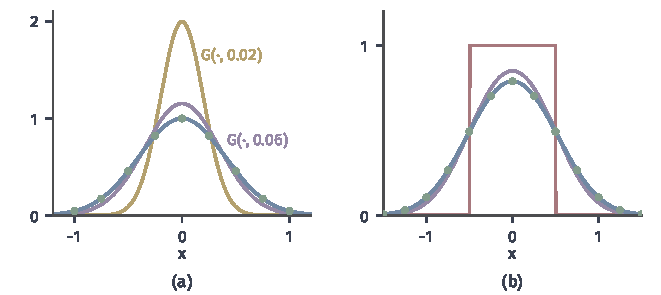
\includegraphics[width=112mm]{figures/06-differential-equations/02-partial-differential-equations/matplotlib/heat-semigroup-composition/figure.pdf}
  \caption{时间拼接。(a)$G(\cdot,0.02)$（黄）与$G(\cdot,0.06)$（紫）的数值卷积（绿点）落在$G(\cdot,0.08)$（蓝）上。(b)方框（红）先走$0.06$（紫）再走$0.02$（绿点），与一步走$0.08$的解（蓝）一致。}
  \label{fig:heat-semigroup-composition}
\end{BookInlineFigure}

\paragraph{强连续半群}
把这些性质抽象出来。注意其中只有$t\geq0$，反向一般不存在，这是“半”字的含义。

\begin{definition}[强连续半群]
\label{def:heat-c0-semigroup}
设$X$是Banach空间，$\{S(t)\}_{t\geq0}$是$X$上的有界线性算子族。若
\begin{equation}
 S(0)=I,\qquad S(t+s)=S(t)S(s),\qquad \lim_{t\to0^+}\lVert S(t)x-x\rVert_X=0
 \label{eq:heat-c0-semigroup}
\end{equation}
对所有$t,s\geq0$和$x\in X$成立，则称它是\term{强连续半群}（strongly continuous semigroup）。若还有$\lVert S(t)\rVert\leq1$，称为\term{压缩半群}（contraction semigroup）。把$u_0$映到解的这样一族算子称为\term{解半群}（solution semigroup）。
\end{definition}

强连续是一个与空间有关的性质，这正是上一节初值恢复定理的用武之地。由定理~\ref{thm:heat-uniform-recovery}和定理~\ref{thm:heat-lp-recovery}，全空间热半群在$C_0(\mathbb{R}^{d})$、有界一致连续函数空间及$L^p$（$1\leq p<\infty$）上是强连续的压缩半群；这里用到的是$S(t)$把这些空间映到自身，$C_0$的情形可由控制收敛定理得到。在$L^\infty$上$S(t)$仍是压缩的半群，却不强连续，$\operatorname{sign}(x)$就是反例。

强连续只要求对每个固定的$x$收敛，不要求算子范数收敛。对区间上的$L^2$半群，算子是对角的，所以
\[
 \lVert S(t)-I\rVert=\sup_k\bigl(1-\mathrm{e}^{-\lambda_kt}\bigr)=1,\qquad t>0 .
\]
无论$t$多小，足够高的频率都还没有“被恢复”，图~\ref{fig:heat-unbounded-generator}(a)。对矩阵则$\lVert\mathrm{e}^{t\bm{A}}-\bm{I}\rVert\to0$，这是有限维和无限维的本质差别之一。

\paragraph{生成元}
矩阵可以由指数函数在零点的导数取回：
\[
 \bm{A}=\lim_{t\to0}\frac{\mathrm{e}^{t\bm{A}}-\bm{I}}{t} .
\]
对半群做同样的事，极限只对部分$x$存在。

\begin{definition}[生成元]
\label{def:heat-generator}
设$\{S(t)\}$是$X$上的强连续半群。对$x\in X$考虑差商的极限
\begin{equation}
 Ax=\lim_{t\to0^+}\frac{S(t)x-x}{t} .
 \label{eq:heat-generator-limit}
\end{equation}
使这个极限在$X$中存在的$x$构成子空间$D(A)$。称$A$为半群的\term{生成元}（generator），$D(A)$为它的定义域。
\end{definition}

区间上的情形可以完全算出来，而且把边界条件的位置显露出来。

\begin{theorem}[区间热半群的生成元]
\label{thm:heat-generator}
在$X=L^2(0,1)$上，设$S(t)$是零Dirichlet条件的半群，$u=\sum_kc_ke_k$。则
\begin{equation}
 D(A)=\Bigl\{u:\sum_k\lambda_k^2c_k^2<\infty\Bigr\}=H^2(0,1)\cap H^1_0(0,1),\qquad Au=u'' .
 \label{eq:heat-generator-dirichlet}
\end{equation}
零Neumann条件时，用$\tilde{e}_k$的坐标写同样的条件，得到
\begin{equation}
 D(A)=\{u\in H^2(0,1):u'(0)=u'(1)=0\},\qquad Au=u'' .
 \label{eq:heat-generator-neumann}
\end{equation}
\end{theorem}

\begin{proof}
只写Dirichlet情形，Neumann情形把正弦换成余弦，并加上$k=0$一项。

设$\sum_k\lambda_k^2c_k^2<\infty$，令$y=-\sum_k\lambda_kc_ke_k$。按坐标计算
\[
 \Bigl\lVert\frac{S(t)u-u}{t}-y\Bigr\rVert_2^2=\sum_k\Bigl(\frac{\mathrm{e}^{-\lambda_kt}-1}{t}+\lambda_k\Bigr)^2c_k^2 .
\]
由$0\leq1-\mathrm{e}^{-\lambda t}\leq\lambda t$，括号中的量属于$[0,\lambda_k]$，每一项不超过可和的$\lambda_k^2c_k^2$，又对每个$k$趋于零。由控制收敛定理，和趋于零，所以$u\in D(A)$且$Au=y$。

反过来，若极限$y$存在，取第$k$个坐标，$\langle y,e_k\rangle=-\lambda_kc_k$，由Parseval等式，$\sum_k\lambda_k^2c_k^2$等于$\lVert y\rVert_2^2$，有限。

现在识别这个集合。若$\sum_k\lambda_k^2c_k^2<\infty$，部分和$u_N$在$H^2$中是Cauchy列，因为
\[
 \lVert u_N''\rVert_2^2=\sum_{k\leq N}\lambda_k^2c_k^2,\qquad \lVert u_N'\rVert_2^2=\sum_{k\leq N}\lambda_kc_k^2 .
\]
极限$u\in H^2$，$H^1$收敛蕴含端点值收敛，所以$u(0)=u(1)=0$，且$u''=-\sum_k\lambda_kc_ke_k=y$。

若$u\in H^2\cap H^1_0$，分部积分两次，端点项因$u$和$e_k$在两端为零而消失，
\[
 \langle u'',e_k\rangle=\langle u,e_k''\rangle=-\lambda_kc_k .
\]
由Parseval等式，$\sum_k\lambda_k^2c_k^2$等于$\lVert u''\rVert_2^2$，有限。
\end{proof}

这个定理说明，两种边界条件对应同一个微分表达式$u''$，却是两个不同的算子，图~\ref{fig:heat-generator-domain}。边界条件不在表达式里，而在定义域里。前面分离变量时边界条件决定可用的模式，这里是同一件事的算子语言。

\begin{BookInlineFigure}
  \centering
  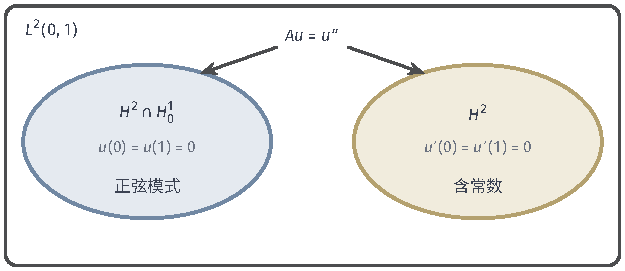
\includegraphics[width=105mm]{figures/06-differential-equations/02-partial-differential-equations/tikz/heat-generator-domain/figure.pdf}
  \caption{同一个表达式$Au=u''$的两个定义域，都是$L^2(0,1)$的稠密子空间。左（蓝）是零Dirichlet条件，由正弦模式张成；右（黄）是零Neumann条件，包含常数，生成不同的半群。}
  \label{fig:heat-generator-domain}
\end{BookInlineFigure}

生成元是无界算子：$\lVert Ae_k\rVert_2=k^2\pi^2\to\infty$，这也是$\lVert S(t)-I\rVert$不趋于零的原因。于是$\mathrm{e}^{tA}$不能用幂级数定义，一般的$u\in L^2$根本不在$D(A^n)$中。空间离散后，这种无界性表现为矩阵最大特征值随网格加细而增长，约为$4/h^2$，图~\ref{fig:heat-unbounded-generator}(b)。

\begin{BookInlineFigure}
  \centering
  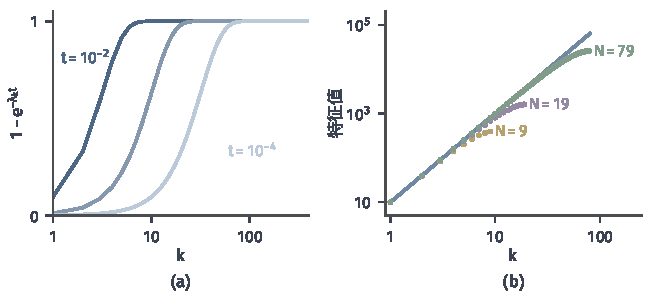
\includegraphics[width=112mm]{figures/06-differential-equations/02-partial-differential-equations/matplotlib/heat-unbounded-generator/figure.pdf}
  \caption{生成元的无界性。(a)$1-\mathrm{e}^{-\lambda_kt}$对$k$的关系，$t=10^{-2},10^{-3},10^{-4}$（蓝色由深到浅），对每个$t$都随$k$增大趋于$1$。(b)离散Laplace矩阵的特征值$4h^{-2}\sin^2(k\pi h/2)$，$N=9,19,79$（点），蓝线是$\lambda_k=k^2\pi^2$，网格越细能到达的特征值越大。}
  \label{fig:heat-unbounded-generator}
\end{BookInlineFigure}

\paragraph{一般区域与源项}
一般的有界区域上，可以用第~\ref{chap:elliptic-equations}章的双线性型定义生成元。令
\[
 a(u,v)=\int_\Omega\nabla u\cdot\nabla v\,\mathrm{d}\bm{x} .
\]
$D(A)$由这样的$u\in H^1_0(\Omega)$组成：存在$g\in L^2(\Omega)$，使$a(u,v)=-\langle g,v\rangle$对所有$v\in H^1_0(\Omega)$成立，此时$Au=g$。Dirichlet边界藏在空间$H^1_0$里，$g$是弱意义下的$\Delta u$。

$-A$的逆是椭圆问题的解算子，它在$L^2(\Omega)$上紧且自伴。由紧自伴算子的谱定理，存在$L^2(\Omega)$的标准正交基$\{e_k\}$和$0<\lambda_1\leq\lambda_2\leq\cdots\to\infty$，于是半群可以直接写成
\begin{equation}
 S(t)u_0=\sum_k\mathrm{e}^{-\lambda_kt}\langle u_0,e_k\rangle e_k ,
 \label{eq:heat-spectral-semigroup}
\end{equation}
谱定理可参考\BookChapterRef{chap:operator-spectra}{卷四第18章“算子谱”}。一般的算子何时生成半群由Hille--Yosida定理回答，它的证明需要预解式的估计，这里的算子已经有了显式的谱表示，所以用不到它。

源项的公式回到前面的切片思想。设$f:[0,T]\to X$连续，
\begin{equation}
 u(t)=S(t)u_0+\int_0^tS(t-s)f(s)\,\mathrm{d}s
 \label{eq:heat-mild}
\end{equation}
称为\term{温和解}（mild solution）。它只要求半群存在，而不要求$u$可微。强连续性和$\lVert S(t)\rVert\leq1$保证被积函数连续，积分在$X$中存在。数据足够好时，它与经典解一致，式~\eqref{eq:heat-duhamel-space}和式~\eqref{eq:heat-duhamel-modes}是它的两个具体形式。

最后，半群和椭圆问题之间有一个简单的关系。在零Dirichlet的情形下，把式~\eqref{eq:heat-spectral-semigroup}对时间从$0$积到$\infty$，每个模式的因子积分为$1/\lambda_k$，所以对$f\in L^2(\Omega)$，
\[
 \int_0^\infty S(t)f\,\mathrm{d}t=(-A)^{-1}f .
\]
恒定热源在无穷长时间内累积的响应，就是Poisson问题的解。例~\ref{ex:heat-source-steady}中$a_k\to f_k/\lambda_k$是这个等式的坐标形式。

与矩阵的对照见表~\ref{tab:heat-matrix-analogy}。

\begin{BookInlineTable}
  \centering
  \caption{矩阵指数与热半群的对照。}
  \label{tab:heat-matrix-analogy}
  \begin{tabular}{lll}
    \toprule
    & 线性常微分方程 & 热方程\\
    \midrule
    演化算子 & $\mathrm{e}^{t\bm{A}}$，$t\in\mathbb{R}$ & $S(t)$，$t\geq0$\\
    生成元 & 有界，处处有定义 & 无界，定义域含边界条件\\
    小时间连续 & 按算子范数 & 只按每个初值\\
    输入响应 & 常数变易公式 & Duhamel公式（温和解）\\
    \bottomrule
  \end{tabular}
\end{BookInlineTable}
